% % This template is provided for all the participants of the seminar ``Social Network Data Analytics''
%%%%%%%%%%%%%%%%%%%%%
% Author information:
%%%%%%%%%%%%%%%%%%%%%
% Jannik Strötgen
% Institute of Computer Science
% Database Systems Research Group
% INF 348
% 69120 Heidelberg
% stroetgen@uni-hd.de
%%%%%%%
% Date: April 24, 2010
% minor modifications: October 17, 2011
%%%%%%%

\documentclass[
     11pt,         % font size
     a4paper,      % paper format
     oneside,
     ]{article}

%%%%%%%%%%%%%%%%%%%%%%%%%%%%%%%%%%%%%%%%%%%%%%%%%%%%%%%%%%%%

% PACKAGES:

% Use German :
\usepackage[USenglish, ngerman]{babel}
% Input encoding
\usepackage[utf8]{inputenc}
% Font encoding
\usepackage[T1]{fontenc}
% Einbinden von URLs:
\usepackage{url}
% hyperrefs in the documents
\usepackage[bookmarks=true,colorlinks,pdfpagelabels,pdfstartview = FitH,bookmarksopen = true,bookmarksnumbered = true,linkcolor = black,plainpages = false,hypertexnames = false,citecolor = black,urlcolor=black]{hyperref}
%\usepackage{hyperref}
% Include Graphic-files:
\usepackage{graphicx}
% Include PDF links
%\usepackage[pdftex, bookmarks=true]{hyperref}
% Fuer Textsatz
\usepackage{setspace}
% For bibliography style
\usepackage[numbers]{natbib}
% for Latex symbols
\usepackage{doc}
\usepackage{csquotes}
\usepackage{stackengine}
\usepackage{amsmath}
\usepackage{array}
\usepackage{verbatim}
\usepackage{float}

\addto{\captionsngerman}{%
  \renewcommand*{\contentsname}{Contents}
  \renewcommand*{\listfigurename}{Figure}
  \renewcommand*{\listtablename}{Table}
  \renewcommand*{\figurename}{Figure}
  \renewcommand*{\tablename}{Tab.}
}

%%%%%%%%%%%%%%%%%%%%%%%%%%%%%%%%%%%%%%%%%%%
% Titel, Autor, Seminar, Semester, Dozent %
%%%%%%%%%%%%%%%%%%%%%%%%%%%%%%%%%%%%%%%%%%%
\newcommand{\mytitle}{Image Completion Methods}
\newcommand{\myauthor}{Jan Sieber}
\newcommand{\myseminar}{Object Recognition and Image Understanding}
\newcommand{\mysemester}{Summer Semester 2018}
\newcommand{\mydozent}{Prof. Dr. Björn Ommer}
\newcommand{\mydozentTwo}{}
\newcommand{\mydozentThree}{}
\newcommand{\mydozentFour}{}
\newcommand{\mydozentFive}{}
\newcommand{\myMatrikelnummer}{3219317}
\newcommand{\myStudiengang}{Applied Computer Science }
\newcommand{\mySemester}{10}
\newcommand{\myEmail}{uni@email-master.de}



\newcommand{\generalDate}{23.07.2018}

% OTHER SETTINGS:
\setlength{\parindent}{0in}

% Pagestyle:
\pagestyle{myheadings}
\markright{\myauthor: \mytitle}

\begin{document}

%%%%%%%%%%%%%%%%%%%%%%%%%%%%%%%%%%%%% <TITLE> %%%%%%%%%%%%%%%%%%%%%%%%%%%%%%%%%%%%%
\pagenumbering{roman}
\begin{titlepage}
\begin{tabular}[l]{l}
% Angaben zum Seminar
Ruprecht-Karls-Universität Heidelberg\\
Institute of Computer Science\\
\mysemester\\
Report: \myseminar\\
Lecturer: \mydozent\\
\phantom{Dozenten: }\mydozentTwo\\
\phantom{Dozenten: }\mydozentThree\\
\phantom{Dozenten: }\mydozentFour\\
\phantom{Dozenten: }\mydozentFive\\
\end{tabular}

\vspace{4cm}
\begin{center}
\textbf{\large Report} % Proseminararbeit,Studienarbeit, Interdisziplinaeres Projekt
\vspace{0.5\baselineskip}

% Titel wird ausgegeben (siehe oben)
{\huge
\mytitle
}
\end{center}

\vfill
% Persönliche Angaben
\begin{tabular}[l]{ll}
Name:           & \myauthor\\
Matriculation number: & \myMatrikelnummer\\
Course of studies:    & \myStudiengang (\mySemester.\ semester)\\
Email: & \myEmail\\
Date of submission: & \generalDate \\
\end{tabular}

\end{titlepage}
%%%%%%%%%%%%%%%%%%%%%%%%%%%%%%%%%%%%% </TITLE> %%%%%%%%%%%%%%%%%%%%%%%%%%%%%%%%%%%%

% Zeilenabstand
\onehalfspacing


%%%%%%%%%%%%%%%%%%%%%%%%%%%%% <Antiplagiatserklärung> %%%%%%%%%%%%%%%%%%%%%%%%%%%%%

%%%%%%%%%%%%%%%%%%%%%%%%%%%%% <Declaration of Authorship> %%%%%%%%%%%%%%%%%%%%%%%%%%%%%
\hspace*{-1.5in}

\thispagestyle{empty}
\section*{Declaration of Authorship}
\vspace*{100pt}
I, \textbf{\myauthor} hereby confirm that the report I am submitting on \textbf{\mytitle}, in the course \textbf{\myseminar}, is solely my own work. If any text passages or images from books, papers,
the Web or other sources have been copied or in any other way used, all references have been acknowledged and fully cited.
I declare that no part of the report submitted has been used for any other report, thesis or course in
another higher education institution, research institution or educational institution. I am aware of the University's regulations concerning
plagiarism, including those regulations concerning disciplinary actions that may result from plagiarism.
\vspace*{50pt}

Heidelberg, \generalDate \hspace{2cm} \underline{
\includegraphics[scale=0.2]{images/unterschrift.PNG}}
\newpage




\newpage
%%%%%%%%%%%%%%%%%%%%%%%%%%%%% </Declaration of Authorship> %%%%%%%%%%%%%%%%%%%%%%%%%%%%
\section*{Preamble}


\newpage
%%%%%%%%%%%%%%%%%%%%%%%%%%%%%% <Inhaltsverzeichnis> %%%%%%%%%%%%%%%%%%%%%%%%%%%%%%%
% Table of contents
\tableofcontents
\newpage
%%%%%%%%%%%%%%%%%%%%%%%%%%%%%% </HAUPTTEIL> %%%%%%%%%%%%%%%%%%%%%%%%%%%%%%

\pagenumbering{arabic}
\section{Introduction}
Nowadays image processing is getting more and more important. This manifests in many different fields of image processing reaching from classification to image generation.
This project will cover the field of image completion. Due to this field tries to produce new information for an occluded image, it can also be solved by image generation.
Therefore one has several methods available to solve this task. For example variational autencoders or generative adversarial networks. Still, generating images is not the only way to solve this problem. That is why this report will cover three methods and compare them.
\begin{itemize}
  \item Image Stitching
  \item Variational Autoencoders (VAE)
  \item Deep Feature Interpolation (DFI)
\end{itemize}
While the variational autoencoder can be used to generate specific completely new data, DFI and image stitching are not able to do this.
In our examples the MNIST and \enquote{labeled faces in the wild} (LFW) datasets are used. While MNIST has several classes, LFW only consists out of faces. \\
The simplest of the three approaches is \textbf{image stitching}, which just tries to find a similar image according to features and tries to find a transformation of facial landmark coordinates from the nearest neighbor image to the occluded image. With help of this transformation the nearest neighbor can be transformed and the fill the missing parts of the occluded image.\\
The \textbf{variational autoencoder} approach can be trained and then used to
\begin{itemize}
  \item generate a new image and fill the missing parts (trained without occlusion) or
  \item can be trained with the occluded images to reconstruct the missing parts directly (kind of deep learning only).
\end{itemize}
For the generation approach there needs to be an adaption for label specific generation, which will be presented lateron. \\
The \textbf{DFI} approach takes two datasets, which are occluded and not occluded images. According to this the method computes the difference between those two sets in a feature space and adds this difference to the image one wants to reconstruct/complete. Afterwards one needs to reconstruct the image from the feature space. For this backpropagation will be applied to the input.

\section{Convolutional Neural Networks}
Convolutional neural networks are a very important tool to accomplish the goal of image completion for all three methods. Even if convolutional neural networks should be known by almost everyone in this field, one will give a \underline{\textbf{brief}} introduction to CNNs and how it is trained. Afterwards the structure of a VGG19 will be presented, which is a commonly used network and will be used for the algorithms.
\subsection{Structure}
There are several types of layers which can be used to build a CNN.
\subsubsection{Convolution}
The classic convolution is defined by so called \textbf{filters}. Filters can be seen as a window of a specific pixel size, the so called \textbf{kernel size}. This window is moved over the input image. While this process each pixel within this window gets weighted, summed up and therefore produces a single output \enquote{pixel}. This is done for the whole input image. The weight is defined by the kernel weights. For example a filter with kernel size 3x3 has 3*3=9 weights.
\begin{figure}[H]
  \begin{center}
    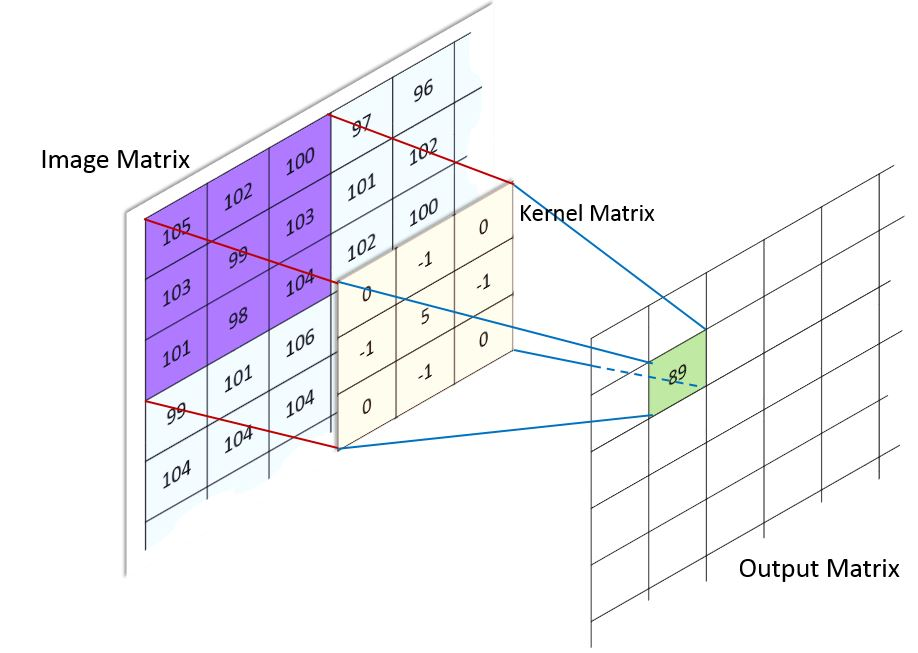
\includegraphics[width=0.5\textwidth]{images/1.JPG}
    \caption{A convolution with kernel size 3x3 producing a single output. The kernel matrix would be slided over the image matrix for further values. The window would be moved to the right for the next value. After the line is finished it would be moved one down, resulting in a slide from left to right and top to bottom.}
    \label{fig:conv}
  \end{center}
\end{figure}

\subsubsection{Pooling}
The pooling layer consists out of a pooling size analogous to the kernel size. In contrast to the filters it has no weights. The window with the pooling size is slided over the input image with a stride (often matching the pooling size). This means, that width and height is halfed with an pooling size of two. Each of these slides produces a single output value.\\
The most common computation is the max-pooling, where the maximum value within this window is taken as output. Still, there are other pooling functions like average pooling or median pooling.
\begin{figure}[H]
  \begin{center}
    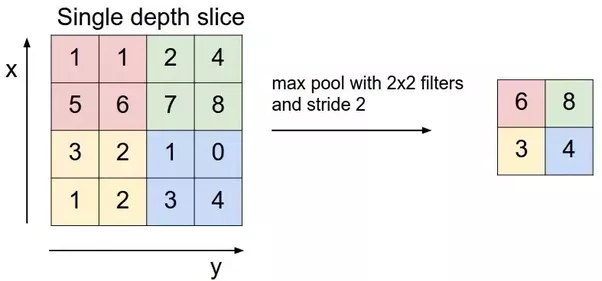
\includegraphics[width=0.5\textwidth]{images/pooling.png}
    \caption{Max-Pooling with size 2 and stride 2.}
    \label{fig:pool}
  \end{center}
\end{figure}

\subsubsection{Fully Connected}
Fully connected (=FC) layers take inputs $x_i$ and compute multiple output values. FC layers consist out of multiple so called \enquote{neurons}. Each of these neurons take every $x_i$ as input and produces a single output $y$. For this process each of these neurons has weights $w_i$. The input $x_i$ is weighted with weight $w_i$. Furthermore each neuron has its own weights, indpendent from the other neurons.
The formular for a single neuron would be
\begin{align*}
  a = \sum^n_{i=0} w_i \cdot x_i
\end{align*}
In the end each neuron puts its computed value in an arbitrary \textbf{non-linear} activation function $\phi$ resulting in
\begin{align*}
  y = \phi (a) = \phi ( \sum^n_{i=0} w_i \cdot x_i )
\end{align*}
If one takes many neurons, one gets a fully connected layer. A $n$ neuron FC layer results in n outputs.
\begin{figure}[H]
  \begin{center}
    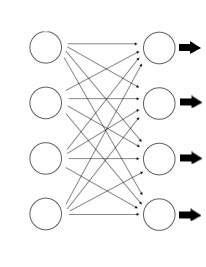
\includegraphics[width=0.3\textwidth]{images/fc-layer.png}
    \caption{Single FC layer. Left circles are the inputs $x_i$, right circles are the neurons producing four outputs.}
    \label{fig:fc-layer}
  \end{center}
\end{figure}

These n outputs now can be taken as input for the next FC layer.
\begin{figure}[H]
  \begin{center}
    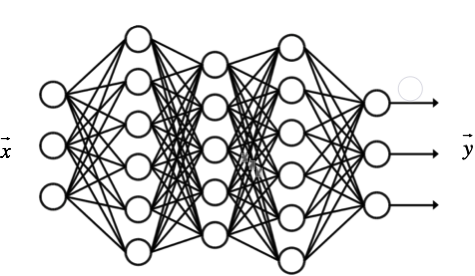
\includegraphics[width=0.5\textwidth]{images/multipleFC.png}
    \caption{Multiple FC layers stacked.}
    \label{fig:multipleFC}
  \end{center}
\end{figure}

\subsubsection{Transposed Convolution}
The transposed convolution is the \enquote{inverse} of the convolutional layer. Even if one calls it the inverse, the process of convolution cannot be inverted mathematically, but it can be inverted according to the shape.
This means, that the output size of the transposed convolution is equal to the input of our convolutional layer and vice versa. To achieve this, one adds zeros at the borders of the input and moves the filter similar to the convolutional process over the image. A stride can be implemented by adding zero paddings between the input pixels.
\begin{figure}[H]
  \begin{center}
    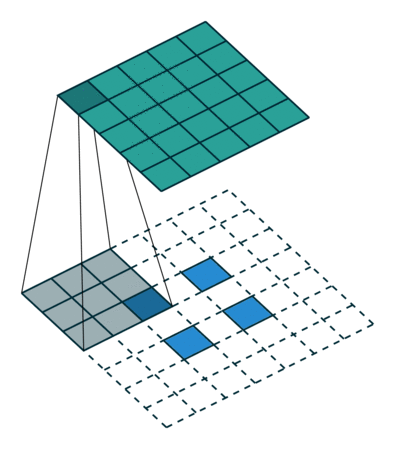
\includegraphics[width=0.4\textwidth]{images/tConv.png}
    \caption{Transposed convolution with no padding, stride of 2 and kernel of 3. Blue is the input, green the output, gray the kernel. One can see the padding between the pixel due to the stride of 2.}
    \label{fig:tConv}
  \end{center}
\end{figure}

\subsection{Learning the Network}
The networks are learned with with the backpropagation algorithm, which is just the chainrule applied to our error function to get the gradients for our weights within the neural network. Explaining this in depth would expand this report for three more pages and would be too much. Visit http://neuralnetworksanddeeplearning.com/ for further information.

\subsection{VGG19}
The VGG19 network is just a network with a defined structure, which is commonly used.
\begin{figure}[H]
  \begin{center}
    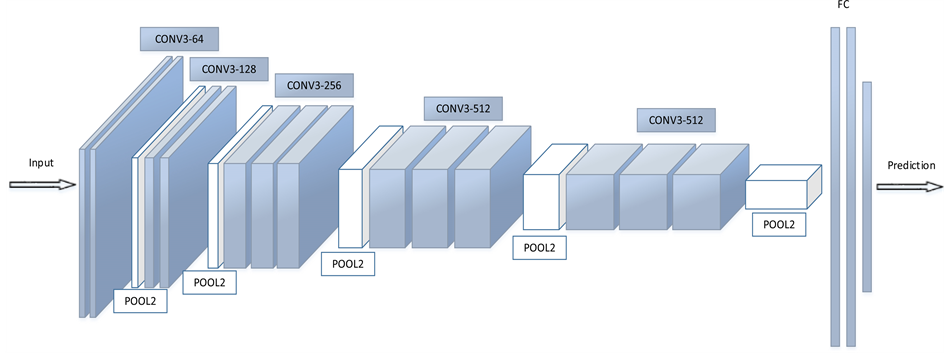
\includegraphics[width=1.0\textwidth]{images/VGG19-orig.png}
    \caption{The VGG-19 network. The specific structure within the convolutional layers is determined by CONV<kernel size>-<number of channels>}
    \label{fig:VGG19-orig}
  \end{center}
\end{figure}
As one can see in figure \ref{fig:VGG19-orig} the network consists out of six major blocks. The first five blocks are multiple convolutional layers followed by a max-pooling layer with kernel size 2. As one can see the first two blocks have two convolutional layers, while the last three blocks have three. The last layer is a triple fully connected output layer with sizes 4096-4096-1000 followed by a softmax layer. Of course the first FC layer is often adapted due to differing image sizes.

\section{ILSVRC 2014}
The \enquote{Imagenet Large Scale Visual Recognition Challenge 2014} is a simple challenge/contest which evaluates CNNs in a large scale for object detection in the year 2014.
Due to the later algorithms use a pretrained network for the ILSVRC 2014, it is useful to know the task of the ILSVRC 2014.
The contest consists out of two major tasks:
\begin{itemize}
  \item Detection
  \item Classification and Localization
\end{itemize}
The dataset for the first task contains 200 basic categories and over 500.000 images which contain over 525.000 objects from these 200 categories.\\
The dataset for the second task contains 1000 categories and over 150.000 images with presence or absence of the objects.\\

\section{Feature extraction}
The feature extraction of an image can be of any type. For example one can take the HOG descriptor and extract features or just use facial landmarks.\\
In this project the feature vectors are extracted from an intermediate layer of a CNN, which is a pretrained VGG-19 on the ILSVRC 2014.
One just forwardpasses the image and takes the vectorized/flattened representation of the output of intermediate layers.
This vector is now our feature vector which represents the image. In case of an 3x3x64 convolutional layer output, the feature vector would be of size 1x576 $\equiv$ 1x(3*3*64).\\
\begin{figure}[H]
  \begin{center}
    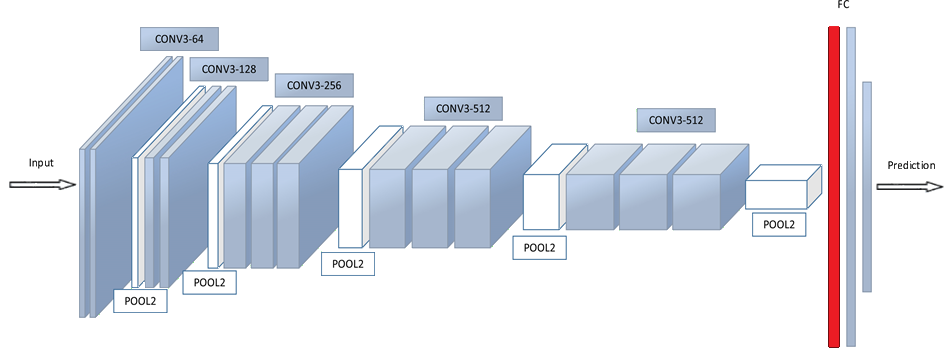
\includegraphics[width=1.0\textwidth]{images/VGG19.png}
    \caption{The VGG-19 network with the first FC layer in red.}
    \label{fig:VGG19}
  \end{center}
\end{figure}
One can see in figure \ref{fig:VGG19} that one took the first FC layer output as our representation in this project.


\section{Nearest neighbor search}
Nearest neighbor search is an easy algorithm to find similar items in a dataset and is used to prefilter the matches lateron. Assume one has a dataset with n items $D = {d_1, d_2, ..., d_n}$ and wants to find the most similar sample $d_i$ to our additional sample $s$. Here $d_i$ and s are feature vectors extractet like described beforehand. All one needs in this case is proper a distance function $\phi(a,b) = x$. This can be for example the manhattan or euclidean distance. \\
The task is then to solve
\begin{align*}
  \text{nearest neighbor} = \underset{x \in D}{argmin} [\phi(s,x)]
\end{align*}
Anologous to the above described one nearest neighbors, for the 100 nearest neighbors one would search for the 100 minimal distances.



\section{Methods}
\subsection{Image Stitching}
The most simple method is image stitching. As stated in the introduction, there are three major parts for this method.
\begin{itemize}
  \item Find the best matching image to the occluded image.
  \item Find a transformation from the best matching image to the occluded image.
  \item Fill in the missing parts.
\end{itemize}
\subsubsection{Finding the Best Image}
The best image is found with the nearest neighbor algorithm. Here the cosine distance function
\begin{align*}
  cosine(a,b) = \frac{\sum^n_{i=1} a_i \cdot b_i}{ \sqrt{\sum^n_{i=1} (a_i)^2} \cdot \sqrt{\sum^n_{i=1} (b_i)^2} }
\end{align*}
is used. It has to be mentioned, that if the vectors are normalized, the cosine distance shortens to
\begin{align*}
  cosine(a,b) = \sum^n_{i=1} a_i \cdot b_i
\end{align*}
, which is the normal manhattan distance. This simplifies computation for the nearest neighbor search. \\
In addition to the cosine distance one can take the pixel loss around the occlusion into account. For this the difference of the pixels around the occlusion is added to the cosine distance resulting in
\begin{align*}
  \phi(a,b)=cosine(a,b)+ \alpha \sum_{c \in C} \sum_{p \in P} |a_{p_c}-b_{p_c}|
\end{align*}
where P contains all direct pixels around the occlusion, a is the nearest neighbor image, b the occluded image, $\alpha$ the importance factor of the pixels color difference and C the channels of the image. This ensures, that colors of the NN is as similar as possible.

\subsubsection{Transformation}
Now a transformation can be found for a linear transformation problem. For this one extracts the facial landmark positions in both pictures and tries to find an optimal linear transformation with the RANSAC algorithm. This also can be done for the color domain of the image (=only for some pixels around the occlusion). With help of these transformations one tries to make the images as similar as possible.

\subsubsection{Stitching}
Now that one has the most similar and transformed image, one can just cut the missing area out of this image and paste it into our occluded image into the same area.

\subsection{Variational Autoencoder}
The second method used is a variational autoencoder. In the following an introduction to VAEs is given and will then be extended to the use with class labels. This has the advantage one does not have to train a VAE for each class, but can use a single VAE for many classes.
\subsubsection{Structure}
A VAE consists out of two major parts, an \textbf{encoder} and \textbf{decoder}. The encoder takes an image as input and reduces this image into an intermediate representation. The decoder then takes this intermediate representation and tries to reconstruct the image matching to this representation. The simplest VAEs consist out of fully connected layers. The more advanced ones use convolutional layers too. It is important that one does not use pooling layers due to pooling layers destroy image information and would result in a \textbf{much} more blurry or incorrect reconstruction. \\
Due to one uses convolutional layers, one needs to know how to \enquote{reverse} this operation. Therefore transposed convolution (=deconvolution) exists. Ofcourse the name deconvolution is not very correct, because it is not possible to have an inverse for a convolution due to its ambiguity.
\subsubsection{Basic Thought}
The main idea of VAEs is to produce the intermediate representation. This intermediate representation then later can be used to generate completely new samples. Lets denote the probability distribution of the latent variables as $p(z)$ and $p(X)$ as the distribution for the images/inputs. \\
The intermediate representation can be seen as mean and variance of a d-dimensional normal distribution representing the image.
That this is the case one needs to approximate a proper distribution $p(z|X)$ which is bound to a unit gaussian by KL-divergence loss. This guarantees, that one can use the latent variables as mean and variance. This can be notated as followed
\begin{align*}
  KLLoss = D_{KL}[Q(z|X)||P(z|X)]
\end{align*}
One also has a second loss for the reconstructed image. For this the pixel loss between the original and the reconstructed image is added on top of the KL-divergence loss.
\begin{align*}
  PixelLoss = \sqrt{\sum_{i,j} (I_{i,j} - R_{i,j})^2}
\end{align*}
The final loss then is
\begin{align*}
  Loss = KLLoss + PixelLoss
\end{align*}
While the pixelloss is very important for the decoder, the KLLoss is most important for the encoders output of latent variables.
\subsubsection{Generating images}
Now that one knows what is the main idea and how to train the VAE, one needs to know how to generate images. This is easy if one uses the reparametrization trick. Due to the output of the encoder is mean and variance, one just needs to produce d random numbers from a unit gaussian $\epsilon$ and use the formula
\begin{align*}
  z = \mu + \sigma \cdot \epsilon
\end{align*}
where $\mu$ is the mean and $\sigma$ the variance.\\
Then z is the input for our decoder, which reconstructs our generated image.

\subsubsection{Extension to Classes}
Due to one has no control for the classes generate by the VAE, there is a simple extension to this. At the moment the decoder of the VAE tries to learn the distribution $p(X'|z)$, where X' is the reconstructed image. This is extendable to class specific generation, if one just adds the class label (=one hot encoded vector) to the latent vector z. Then the decoder just learns the distribution $p(X'|z,c)$ where c is the additional vector.\\
The good thing is, that one does not even need to know the class. One can take a classification network and just take its softmax output as vector c while training the VAE. This gives us the ability to controle the generation process. Now one just needs to feed-forward the concatenated vector z and c into the decoder and an image according to the label will be generated.\\
This is important for later image completion, because the VAE needs to know an approximate label, which is given by the classification network.

\subsection{Deep Feature Interpolation}
\subsubsection{Overview}
In general one has two datasets. One not occluded image set $D_1$ and one occluded image set $D_2$.
. According to this the overview of the algorithm is as followed.
\begin{itemize}
	\item Get feature vector $\sigma (I_1)$ representation of occluded image $I_1$
	\item Have two datasets $D_1, D_2$.
    \item Find 100 nearest neighbors in both datasets according to feature vector
    \item Get the difference vector between the 100 NN of the occluded set and the ones of the the not occluded set.\\
    \item Add scaled diff to feature vector of occluded image $I_1$
    \begin{align*}
    	target = \sigma (I_1) + \alpha \cdot diff
    \end{align*}
    \item Reconstruct the image according to manipulated feature vector by inversion of neural network
    \begin{itemize}
        \item Forward pass (partial reconstructed) image
        $\implies$ first forwardpass is black image
        \item Compute loss (black box for the moment)
        \item Get gradients w.r.t input image
        \item Manipulate pixels according to gradients
    \end{itemize}
\end{itemize}

\subsubsection{Finding the Nearest Neighbors}
The nearest neighbor search is easily done by the cosine distance as in the image stitching approach.
In difference to image stitching one just uses the cosine distance with normalized feature vectors and no additional pixel difference.\\
Now one just needs the feature vector of our image and find its 100 nearest neighbors (=least distances) \textbf{for each of the two sets}.

\subsubsection{Difference Vector}
After on computed the 100 nearest neighbors with the above distance function, one needs to extract the difference vector between the two datasets.
This is done by computing the mean feature vector for each set based on the 100 nearest neighbors.
\begin{align*}
  \mu_{1/2} = \frac{1}{100} \sum^{100}_{i=1} a^i
\end{align*}
where $a^i$ is the feature vector of the i-th neighbor, $\mu_1$ the mean vector for the negative set and $\mu_2$ the mean vector for the positive set.
Then the difference is computed
\begin{align*}
  \sigma_{diff} = \mu_2 - \mu_1
\end{align*}
and added to the image one wants to manipulate by a weightning factor $\alpha$.
\begin{align*}
  \sigma_{toReconstruct} &= \sigma_{toManipulate} + \alpha \sigma_{diff}\\
  \alpha &= \frac{\beta}{\frac{1}{d} w \cdot w}\\
  \beta &= 0.4
\end{align*}
\subsubsection{Image Reconstruction}
Now that one has the manipulated feature vector $\sigma_{toReconstruct}$ which now contains our completed image in feature vector form, one needs to transform this into an image again. This can be done by inverting the neural network. First a black image is fed forward. Then the feature vector $\sigma_{black}$ for the initially black image is extracted. Afterwards one computes the Loss
\begin{align*}
  Loss = \frac{1}{2} ||\sigma_{toReconstruct} - \sigma_{black}||_2^2
\end{align*}
Then the gradients are added to an initially black input image. This is done 200 times until the image is fully reconstructed. \\
Due to this reconstruction process is very unstable and gradients can explode in some areas, one adds a neighbor pixel loss to the image to smooth the image a bit.
\begin{align*}
  R_V = \sum_{i,j} ((\sigma_{black_{i,j+1}} - \sigma_{black_{i,j}})^2 + (\sigma_{black_{i+1,j}} - \sigma_{black_{i,j}})^2)^{\frac{\beta}{2}}
\end{align*}
This makes the final loss look like the following
\begin{align*}
  Loss = \frac{1}{2} ||\sigma_{toReconstruct} - \sigma_{black}||_2^2 + \lambda R_V
\end{align*}
where $\lambda$ is an image smoothening factor and $\beta = 0.4$ like before.






\section{Experiments and Results}
\subsection{Datasets}
In this project three datasets were used.
\begin{itemize}
  \item MNIST \\
  A handrwitten digit dataset. The digits are normalized, mostly center and transformed into grayscale.
  The image size is 28x28 and the dataset has ten classes (= one for each digit). In this dataset 60.000 training and 10.000 are available.
  \item Labeled faces in the wild (=LFW)\\
  LFW is a face dataset with aligned faces. They are labeled with the person they are displaying, which is more or less unimportant for this work. The dataset is just treated unlabeled. The dataset contains 13233 images.
  \item CIFAR 10
  The CIFAR 10 dataset is dataset contain 10 classe. The 10 classes are: airplane, automobile, bird, cat, deer, dog, frog, horse, ship, truck. The dataset contains 50000 training images and 10000 test images, which are of size 32x32 in RGB mode.
\end{itemize}

\subsection{Structures of networks}
Due to many networks are used, here the network architectures are introduced.
\subsubsection{MNIST classification network}
\begin{figure}[H]
  \begin{center}
    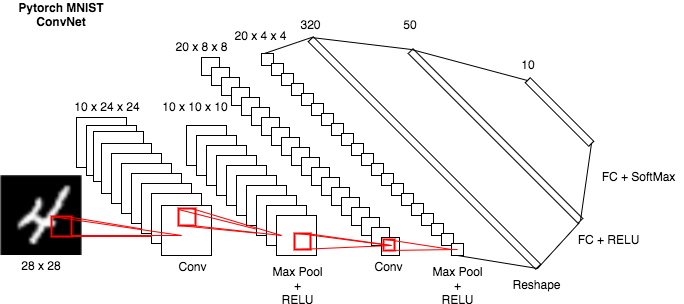
\includegraphics[width=0.5\textwidth]{images/mnist_convet.png}
    \caption{A convolutional neural network to classify MNIST digits.}
  \end{center}
\end{figure}
\subsubsection{VAE on MNIST}
Here one uses only FC layers.
The layer structure is
\begin{itemize}
  \item Vectorized image (image width * image height * number of channels)
  \item 512 neruons
  \item 256 neruons
  \item 64 neruons for variance and 64 for mean.
  \item Reparametrization + MNIST as additional input for the decoder.
  \item 256 neruons
  \item 512 neruons
  \item Reshaped to image (image width * image height * number of channels)
\end{itemize}

\subsubsection{VAE on labeled faces in the wild}
\begin{figure}[H]
  \begin{center}
    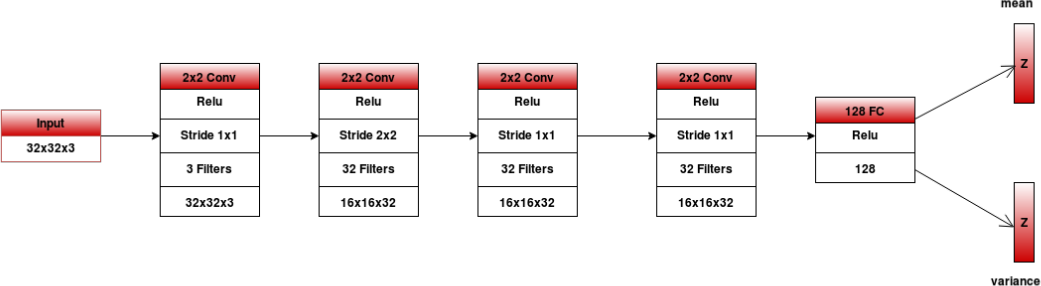
\includegraphics[width=0.5\textwidth]{images/cifar10_encoder.png}
    \caption{The encoder of the VAE for the LFW dataset.}
  \end{center}
\end{figure}
\begin{figure}[H]
  \begin{center}
    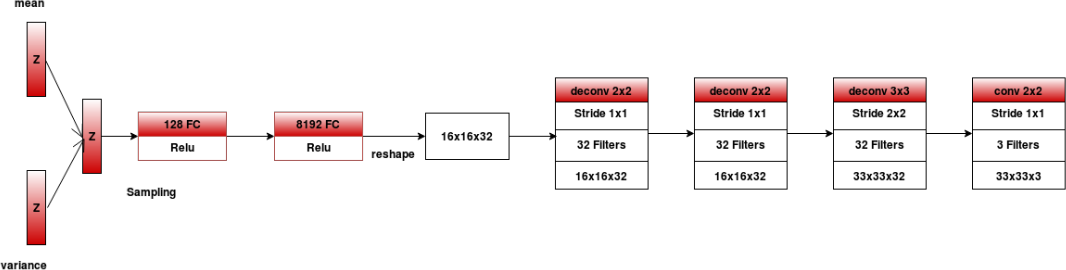
\includegraphics[width=0.5\textwidth]{images/cifar10_decoder.png}
    \caption{The decoder of the VAE for the LFW dataset.}
  \end{center}
\end{figure}

\subsubsection{VGG-19}
\begin{figure}[H]
  \begin{center}
    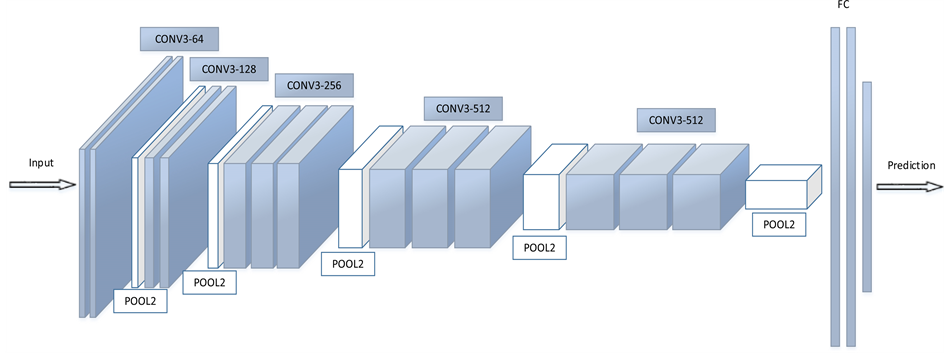
\includegraphics[width=0.5\textwidth]{images/VGG19-orig.png}
    \caption{The VGG-19 network.}
  \end{center}
\end{figure}

\subsection{Image Stitching}
Image stitching is the simplest method. There were not many parameters to adjust. It was just finding the best nearest neighbor and cut \& paste the missing parts.
Still there were different methods tried out from the beginning to find the nearest neighbors.
\begin{itemize}
  \item Nearest neighbor search with faiss index with \textbf{one} result. Stitching without finding the transformation for facial landmarks between two images.
  \item Nearest neighbor search with faiss index with \textbf{100} result images.
  Finding \textbf{one} nearest neighbor out of the 100 with pixel loss around the occluded part. Stitching \textbf{without} finding the transformation for facial landmarks between two images.
  \item Nearest neighbor search with faiss index with \textbf{100} result images.
  Finding \textbf{one} nearest neighbor out of the 100 with pixel loss around the occluded part. Stitching \textbf{with} finding the transformation for facial landmarks between two images.
\end{itemize}
Pixel loss is done as described in the above sections. \\
For the feature vectors for the NN search one needs to differ between the datasets.
\begin{itemize}
  \item MNIST
  \begin{itemize}
    \item VGG-19 pretrained on ILSVRC $\implies$ output of the first FC layer.
    \item Pretrained MNIST classification network from above $\implies$ output of last softmax layer (=used for foinal results).
  \end{itemize}
  \item LFW
  \begin{itemize}
    \item VGG-19 pretrained on ILSVRC $\implies$ output of the first FC layer.
  \end{itemize}
\end{itemize}
The final results (=third method from above) are the following:
  \begin{figure}[H]
    \begin{center}
      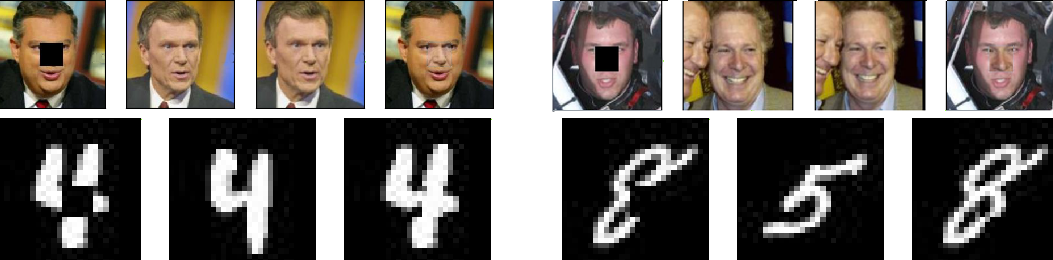
\includegraphics[width=0.8\textwidth]{images/stitching_final2.png}
      \caption{Results for image stitching on LFW and MNIST}
    \end{center}
  \end{figure}


\subsection{Variational Autoencoder}
The VAE method has the most parameters.
\begin{itemize}
  \item The additional input for the decoder. Here one can use which layer of the classification network should be injected into the intermediate representation of the VAE. \textbf{This is only available for the MNIST dataset!}
  \item Use random generation of the VAE or not. Here one can chose if samples should be generated and then stitched into the image or the network just acts as a normal deep learning structure reconstructing the occluded parts directly.
  \item Use the occluded images to train the VAE or not.
\end{itemize}
The results for the MNIST are:
\begin{figure}[H]
  \begin{center}
    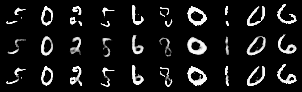
\includegraphics[width=0.8\textwidth]{presentation_results/VAE/MNIST-VAE-useRandom_false-useMNIST_true-VAERepresentation_3-useOccludedForTrain_false.png}
    \caption{Additional input used (softmax output). Did not use random generation (=just deep learning). Used not occluded images for training. First row = occluded image, second row=generated, third row=completed image.}
  \end{center}
\end{figure}
\begin{figure}[H]
  \begin{center}
    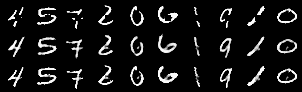
\includegraphics[width=0.8\textwidth]{presentation_results/VAE/MNIST-VAE-useRandom_true-useMNIST_true-VAERepresentation_1-useOccludedForTrain_false.png}
    \caption{Additional input used (flattened vector of last convolutional output). Did not use random generation (=just deep learning). Used not occluded images for training. First row = occluded image, second row=generated, third row=completed image.}
  \end{center}
\end{figure}
One can clearly see, that the preciser/bigger the additional input from the MNIST network gets, the results get better. This is normal due to the encoder relies more and more on the MNIST classification output. \\
Due to this is still just a forward pass (=just deep learning), let's analyse the \textbf{random generation} image completion. Here images are generated and stitched.
\begin{figure}[H]
  \begin{center}
    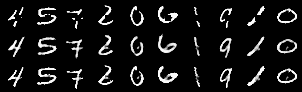
\includegraphics[width=0.8\textwidth]{presentation_results/VAE/MNIST-VAE-useRandom_true-useMNIST_true-VAERepresentation_1-useOccludedForTrain_false.png}
    \caption{Additional input used (flattened vector of last convolutional output). Did use random generation (=just deep learning). Used not occluded images for training. First row = occluded image, second row=generated, third row=completed image.}
  \end{center}
\end{figure}
This version with random generation still can compete with the simple deep learning from above. Still, if one reduces the input from the MNIST classification the results get worse again.
\begin{figure}[H]
  \begin{center}
    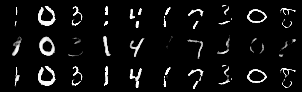
\includegraphics[width=0.8\textwidth]{presentation_results/VAE/MNIST-VAE-useRandom_true-useMNIST_true-VAERepresentation_3-useOccludedForTrain_false.png}
    \caption{Additional input used (softmax output). Did use random generation (=just deep learning). Used not occluded images for training. First row = occluded image, second row=generated, third row=completed image.}
  \end{center}
\end{figure}
Due to decreasing the output to the softmax again, the results rely more on the VAE itself. This can be improved with a longer training time. For these results the VAE and MNIST network was trained for 20 epochs seperately.\\ \ \\
\begin{figure}[H]
  \begin{center}
    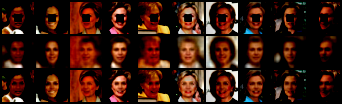
\includegraphics[width=0.8\textwidth]{presentation_results/VAE/LFW-VAE-useRandom_false-useOccludedForTrain_True.png}
    \caption{Did use random generation (=just deep learning). Used occluded images for training.  First row = occluded image, second row=generated, third row=completed image.}
  \end{center}
\end{figure}
\begin{figure}[H]
  \begin{center}
    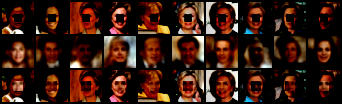
\includegraphics[width=0.8\textwidth]{presentation_results/VAE/LFW-VAE-useRandom_True-useOccludedForTrain_False.png}
    \caption{Did use random generation (=just deep learning). Used occluded images for training.  First row = occluded image, second row=generated, third row=completed image.}
  \end{center}
\end{figure}
The same can be done for the LFW dataset, without additional classification input due to one has no label specific generation.


 Many more parameters has been tried and can be found as images attached as additional folder or generated by modified code.

\subsection{Deep Feature Interpolation}
For the feature vectors for the \textbf{NN search} one needs to differ between the datasets.
\begin{itemize}
  \item MNIST
  \begin{itemize}
    \item VGG-19 pretrained on ILSVRC $\implies$ output of the first FC layer.
    \item Pretrained MNIST classification network from above $\implies$ output of last softmax layer (=used for final results).
  \end{itemize}
  \item LFW
  \begin{itemize}
    \item VGG-19 pretrained on ILSVRC $\implies$ output of the first FC layer.
  \end{itemize}
\end{itemize}
The \textbf{manipulation and reconstruction} of the image is done by using first convolutional layer of the third conv-layer block in the VGG-19 network as described above. \\
The results are the following:
  \begin{figure}[H]
    \begin{center}
      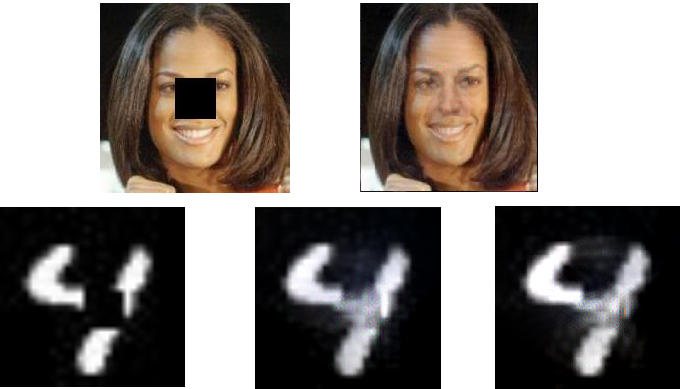
\includegraphics[width=0.8\textwidth]{images/DFI-final2.png}
      \caption{Results for DFI on LFW and MNIST. First MNIST picture=occluded image, second MNIST picture=completed image with feature vectors of VGG-19, third MNIST picture=completed image with feature vectors of MNIST classification network.}
    \end{center}
  \end{figure}
\subsection{Comparison}
While the image stitching and VAE approach perform very well on the MNIST dataset, they more often fail on the LFW dataset. On the LFW dataset the DFI approach is the best solution, while we get some grayish parts due to pollution of the difference vector on the MNIST dataset. This may be fixed with a better feature representation of the MNSIT digits while the NN search.
\cite{dummyEntry}


% References (Literaturverzeichnis):
% a) add ``Literatur'' to table of content
\newpage
\addcontentsline{toc}{section}{Literature}
% b) Style (with abbreviations: use alpha):
\bibliographystyle{plainnat-d}
% c) The File:
\bibliography{seminararbeit}

\end{document}
